%%%%%%%%%%%%%%%%%%%%%%%%%%%%%%%%%%%%%%%%%%%%

%%%%%%%%%%%%%%%%%%%%%%%%%%%%%%%%%%%%%%%%%%%%
% Class options                            %
%%%%%%%%%%%%%%%%%%%%%%%%%%%%%%%%%%%%%%%%%%%%
% Orientation:                             %
% portrait (default), landscape            %
%                                          %
% Paper size:                              %
% a0paper (default), a1paper, a2paper,     %
% a3paper, a4paper, a5paper, a6paper       %
%                                          %
% Language:                                %
% english (default), norsk                 %
%%%%%%%%%%%%%%%%%%%%%%%%%%%%%%%%%%%%%%%%%%%%
\documentclass{uibposter}


\usepackage{lipsum}                                % Dummy text
\usepackage[figwidth = 0.98\linewidth]{todonotes}  % Dummy image (and more!)
\usepackage[absolute, overlay]{textpos}  
\usepackage{varwidth}
\DeclareUnicodeCharacter{200B}{ }% Figure placement
\setlength{\TPHorizModule}{\paperwidth}
\setlength{\TPVertModule}{\paperheight}

% Our packages
\usepackage{tikz}
% tikzscale kann pgfplots skalieren, z.b. zu einem fixen Seitenverhältnis.
\usepackage{tikzscale}
\usepackage{pgfplots}
\pgfplotsset{compat=newest}
\usepgfplotslibrary{external}
% tikzexternalize requires -shell-escape when running latex.
\usetikzlibrary{external}
% exportiere die Bilder in den Ordner tikz
\tikzexternalize[prefix=tikz/]
\DeclareUnicodeCharacter{2212}{−}
\usepgfplotslibrary{groupplots,dateplot}
\usetikzlibrary{patterns,shapes.arrows}
\pgfplotsset{compat=newest}
\def\axisdefaultwidth{8cm}
\def\axisdefaultheight{5cm}
\pgfplotsset{every axis/.style={scale only axis}}

\usepackage{subcaption}

\usepackage{cleveref}


%Library
\usepackage{apacite}
\usepackage{natbib}
\def\bibfont{\scriptsize}
\renewcommand{\bibsection}{\section{Whatever You Prefer}}

\title{The Lax-Wendroff scheme}
\author
{%
    Carla Feistner 
    \and
    Esther Jerez
}
%% Optional:
\institute
{
    Department of mathematics -- University of Bergen
}


% Or:
%\institute{Contact information}


%% Remove footline:
%\setbeamertemplate{footline}{}


\begin{document}

\begin{textblock}{0.5}(0.038, 0.055)
    \color{white}
    \sffamily
    \textbf{Ingress}
    \\
A new second order scheme for hyperbolic conversation laws allowing fast and accurate computation of smooth solutions. 
%TODO Better Impress
%The Lax-Wendroff scheme for solving hyperbolic conservation laws as competitor against the Lax-Friedrichs and Godunov method. Some properties will be presented and the numerical results will be compared.
\end{textblock}

\begin{frame}[fragile]

\begin{columns}
\begin{column}{0.5\textwidth - 1.5cm}
    %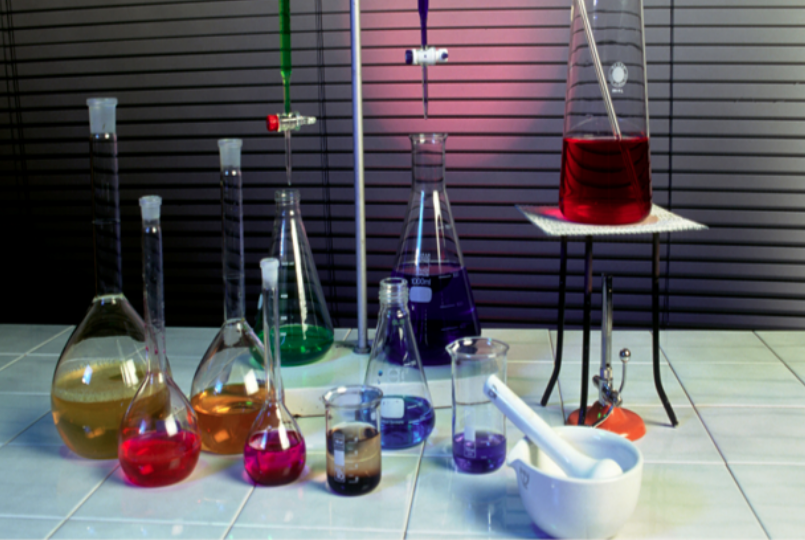
\includegraphics[width = \textwidth]{uibposter-images/bilde1.png}
    %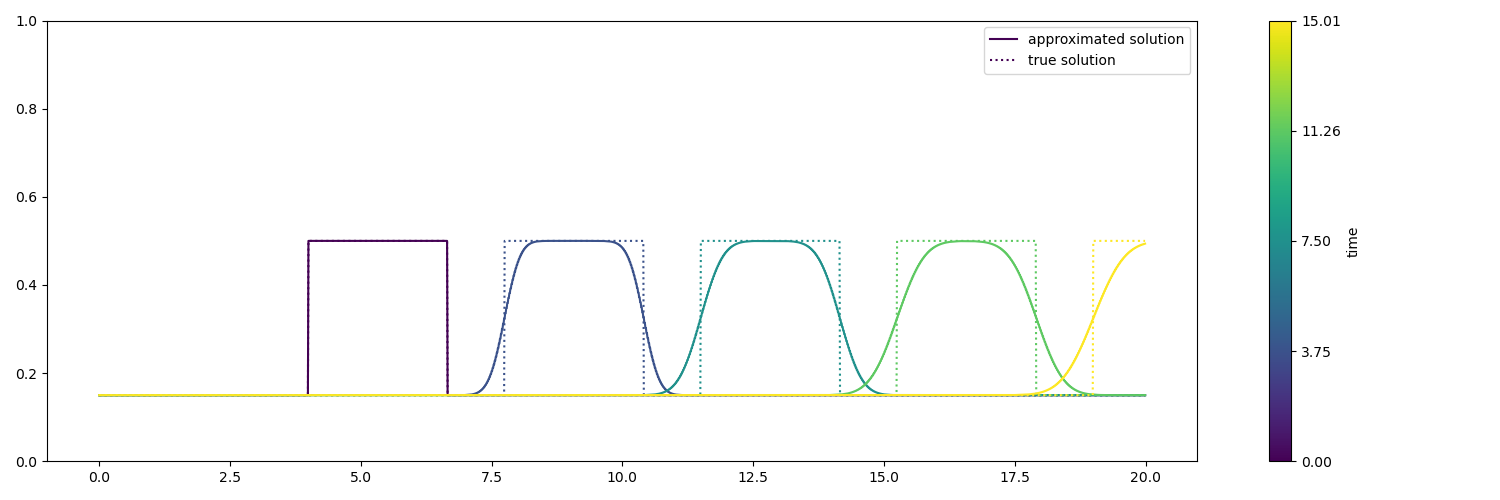
\includegraphics[width=0.95\textwidth, axisratio=7/3]{uibposter-images/test1.tikz}
    \begin{figure}[h]
    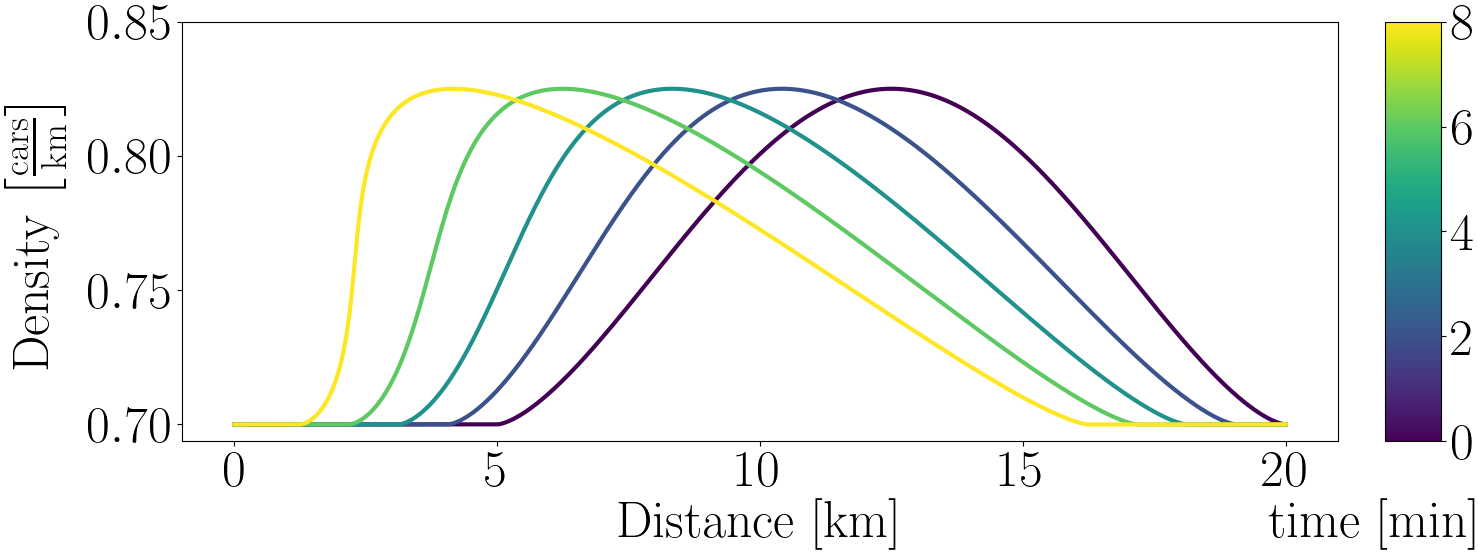
\includegraphics[width=\textwidth]{fig/traffic_motivation_laxW_continous.png} \caption{Build up of a traffic jam produced by the braking of some cars.} \label{img:traffic_flow_motivation}	
    \end{figure}
    \vspace{0.5cm}

\begin{column}{0.5\textwidth - 1.5cm}
\textbf{Abstract}
\vspace{0.5cm}

The main topic of this poster is to introduce the Lax-Wendroff scheme for solving the hyperbolic conservations laws. In concrete, it focus on the 1 space dimensional advection equation for different flows to illustrate how the scheme works, and to compare it with other numerical methods. This will lead us to conclude that the Lax-Wendroff scheme works, in general terms, better than the other ones.

\vspace{0.5cm}
\textbf{Introduction}
\vspace{0.5cm}

Hyperbolic conservation laws are time-dependent systems of partial differential equations that describes the conservation of some quantities. The equation is given as:
\begin{align*}
    u_t + f(u)_x = 0
\end{align*}
Where $u(x,t)$ is a vector of conserved quantities (could be mass, momentum, heat,..) while $f(u)$ is the flux function.

Flux functions are commonly nonlinear functions, leading to nonlinear systems of PDEs where, in general, the exact solution is unknown. Hence numerical methods are used, to compute an approximation. \\
This can be used to simulate traffic jams as we can see in \cref{img:traffic_flow_motivation}. In this case cars are moving from left to right, but as time pass the traffic jam moves in the other direction. 

\end{column}
\begin{column}{0.5\textwidth - 1.5cm}
\textbf{The Lax-Wendroff Method}
\vspace{-1cm}

The general formula of the scheme is given by:
\begin{align*}
&U_j^{n+1} = U_j^n\\
&- \frac{k}{h}\left(f\left(U_{j+\frac{1}{2}}^{n+\frac{1}{2}}\right) - f\left(U_{j-\frac{1}{2}}^{n+\frac{1}{2}}\right)\right)
\end{align*}
where $k$ stepsize in time, $h$ stepsize in space and
\begin{align*}
U_{j+\frac{1}{2}}^{n+\frac{1}{2}} =&~ \frac{1}{2} (U_j^n + U_{j+1}^n)\\
&- \frac{k}{2h}[f(U_{j+1}^n) - f(U_j^n)].
\end{align*}
The step sizes are in the following considered to be controlled by $\frac{k}{h} = const$. This fact is motivated by the CFL condition of the linear case ($u_t + au_x = 0$), where we need $|a|\frac{k}{h} \leq 1$. 
The method can be seen as a concatenation of the Lax-Friderich scheme.
%The computation of the next time step can be written as a function of the solution of the current timestep by $U^{n+1} = \mathcal{H}(U^n)$. This notation can be used to define the local truncation error of a method by
%\begin{align*}
%L_k(x, t) = \frac{u(x, t+k) - \mathcal{H}(u(\cdot, t); x)}{k}
%\end{align*}
%contingent on the used step size in time $k$. This error will now be considered in the linear advection equation with $a > 0$. By Taylor expansion around $u(x, t)$ and some simplifications this yields to:

\vspace{0.5cm}
Computing the local truncation error of the Lax-Wendroff method we obtain
\begin{align*}
L_k(x, t) = \frac{a}{6}(a^2 k^2 - h^2)u_{xxx} + \mathcal{O}(h^3)
\end{align*}
As $L_k(x,t) = \mathcal{O}(h^2)$ the method is consistent and has order 2. Additional for stability the condition $|\nu| < 1$ where $\nu = a\frac{k}{h}$ is the Courant number must be fulfilled. 
In the case of an linear advection equation the convergence of a method follows from consistency and stability by the Lax equivalence theorem. In the nonlinear case Lax and Wendroff proved that a consistent numerical method with bounded solutions always converges to a weak solution of the equation.
The local truncation error also leads to the modified equation which is given as:
\begin{align*}
u_t + a u_x &= \frac{a}{6} (a^2 k^2 - h^2) u_{xxx}\\
&:= \mu u_{xxx}
\end{align*}

    \end{column}
\end{column}
\begin{column}{0.5\textwidth - 1.5cm}
\begin{column}{0.5\textwidth - 1.5cm}
\vspace*{-1.7cm}


This is also a dispersive equation and a solution $u(x, t)$ of it can be represented in Fourier space. By isolating each wavenumber $\xi$ to apply solutions of the form $u(x,t) = e^{i(\xi x - c(\xi)t)}$ to the linear advection equation yields to the dispersion relation:
\begin{align*}
c(\xi) = a\xi + \mu \xi^3
\end{align*}
Based on this relation its possible to calculate the group velocity $c’(\xi)$ for wavenumber $\xi$ which describes in which speed a wave peak travel. It is given by:
\begin{align*}
c'(\xi) = a + 3\mu \xi^2
\end{align*}
As $\mu = \frac{a}{6}h^2(\nu^2 - 1)$ and since $a > 0$ and for stability $|\nu| < 1$ the group velocity $c’(\xi)$ is smaller than $a$ for all $\xi$, but tens to $a$ as $h\rightarrow0$. It follows that the scheme leads to an oscillatory wave train lagging behind the discontinuity, which is traveling with speed $a$. This can also be seen later in the numerical experiments.
    
\vspace{0.5cm}
\textbf{Numerical Analysis}
\vspace{0.5cm}
    
In the following the approximations of the Lax-Wendroff method will be presented in comparison to the Lax-Friedrich and Godunov method.

\vspace{0.5cm}
Applying the methods to the linear advection equation yields to approximations shown in \cref{img:linar_comprehension}. 

\begin{figure}[h]
	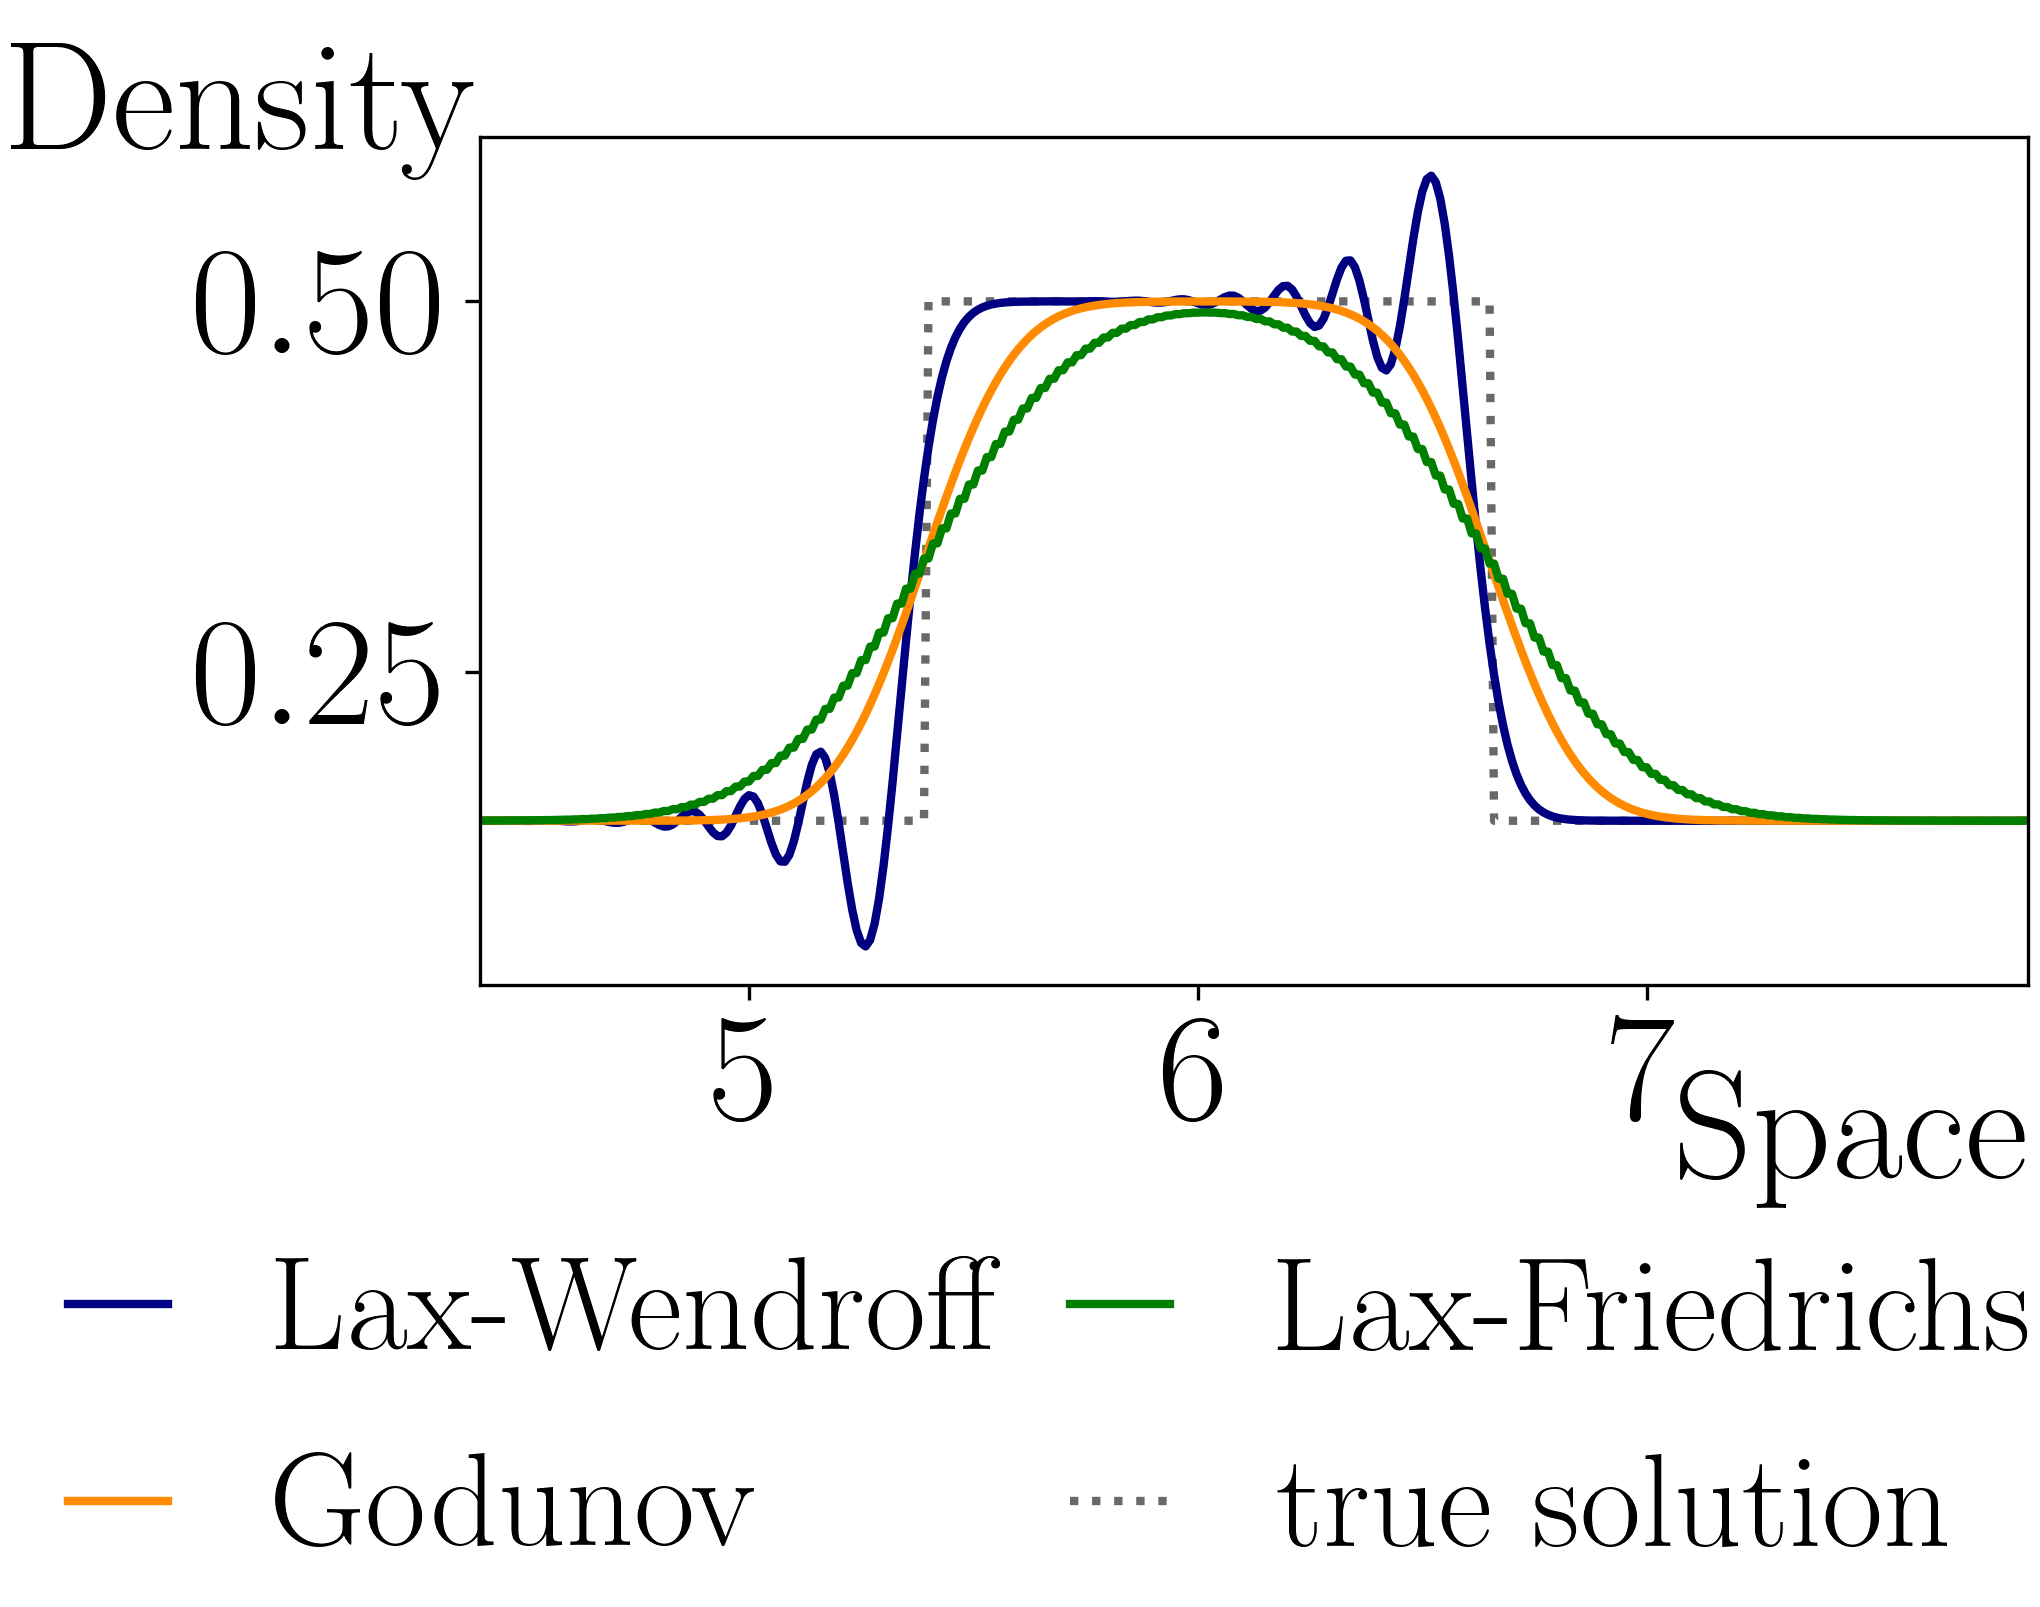
\includegraphics{fig/linear_compare.png}
	\caption{Approximations for the linear advection equation after some time.}
	\label{img:linar_comprehension}
\end{figure}

As comented before the Lax-Wendroff scheme oscilates in front of the discontinuity of the true solution. But on the other hand the discontinuity is approximated better what leads to a smaller error which is shown in \cref{img:error_over_time}. Also notice that the Lax-Friedrich does not reach the 
 
\end{column}
\begin{column}{0.5\textwidth - 1.5cm}
	\vspace*{-1.7cm} 
	
total hight of the true solution resultig in a bad approximation. 

Comparing the runtime of the methods to compute \cref{img:linar_comprehension} turns out that the Gudonov's one is the slowest with a big difference to the others.

\vspace{0.5cm}
Looking deeper into \cref{img:error_over_time} we can confirm that the Lax-Wendroff methods has the lowest error as expected due to its high order.
   
    \begin{figure}
    	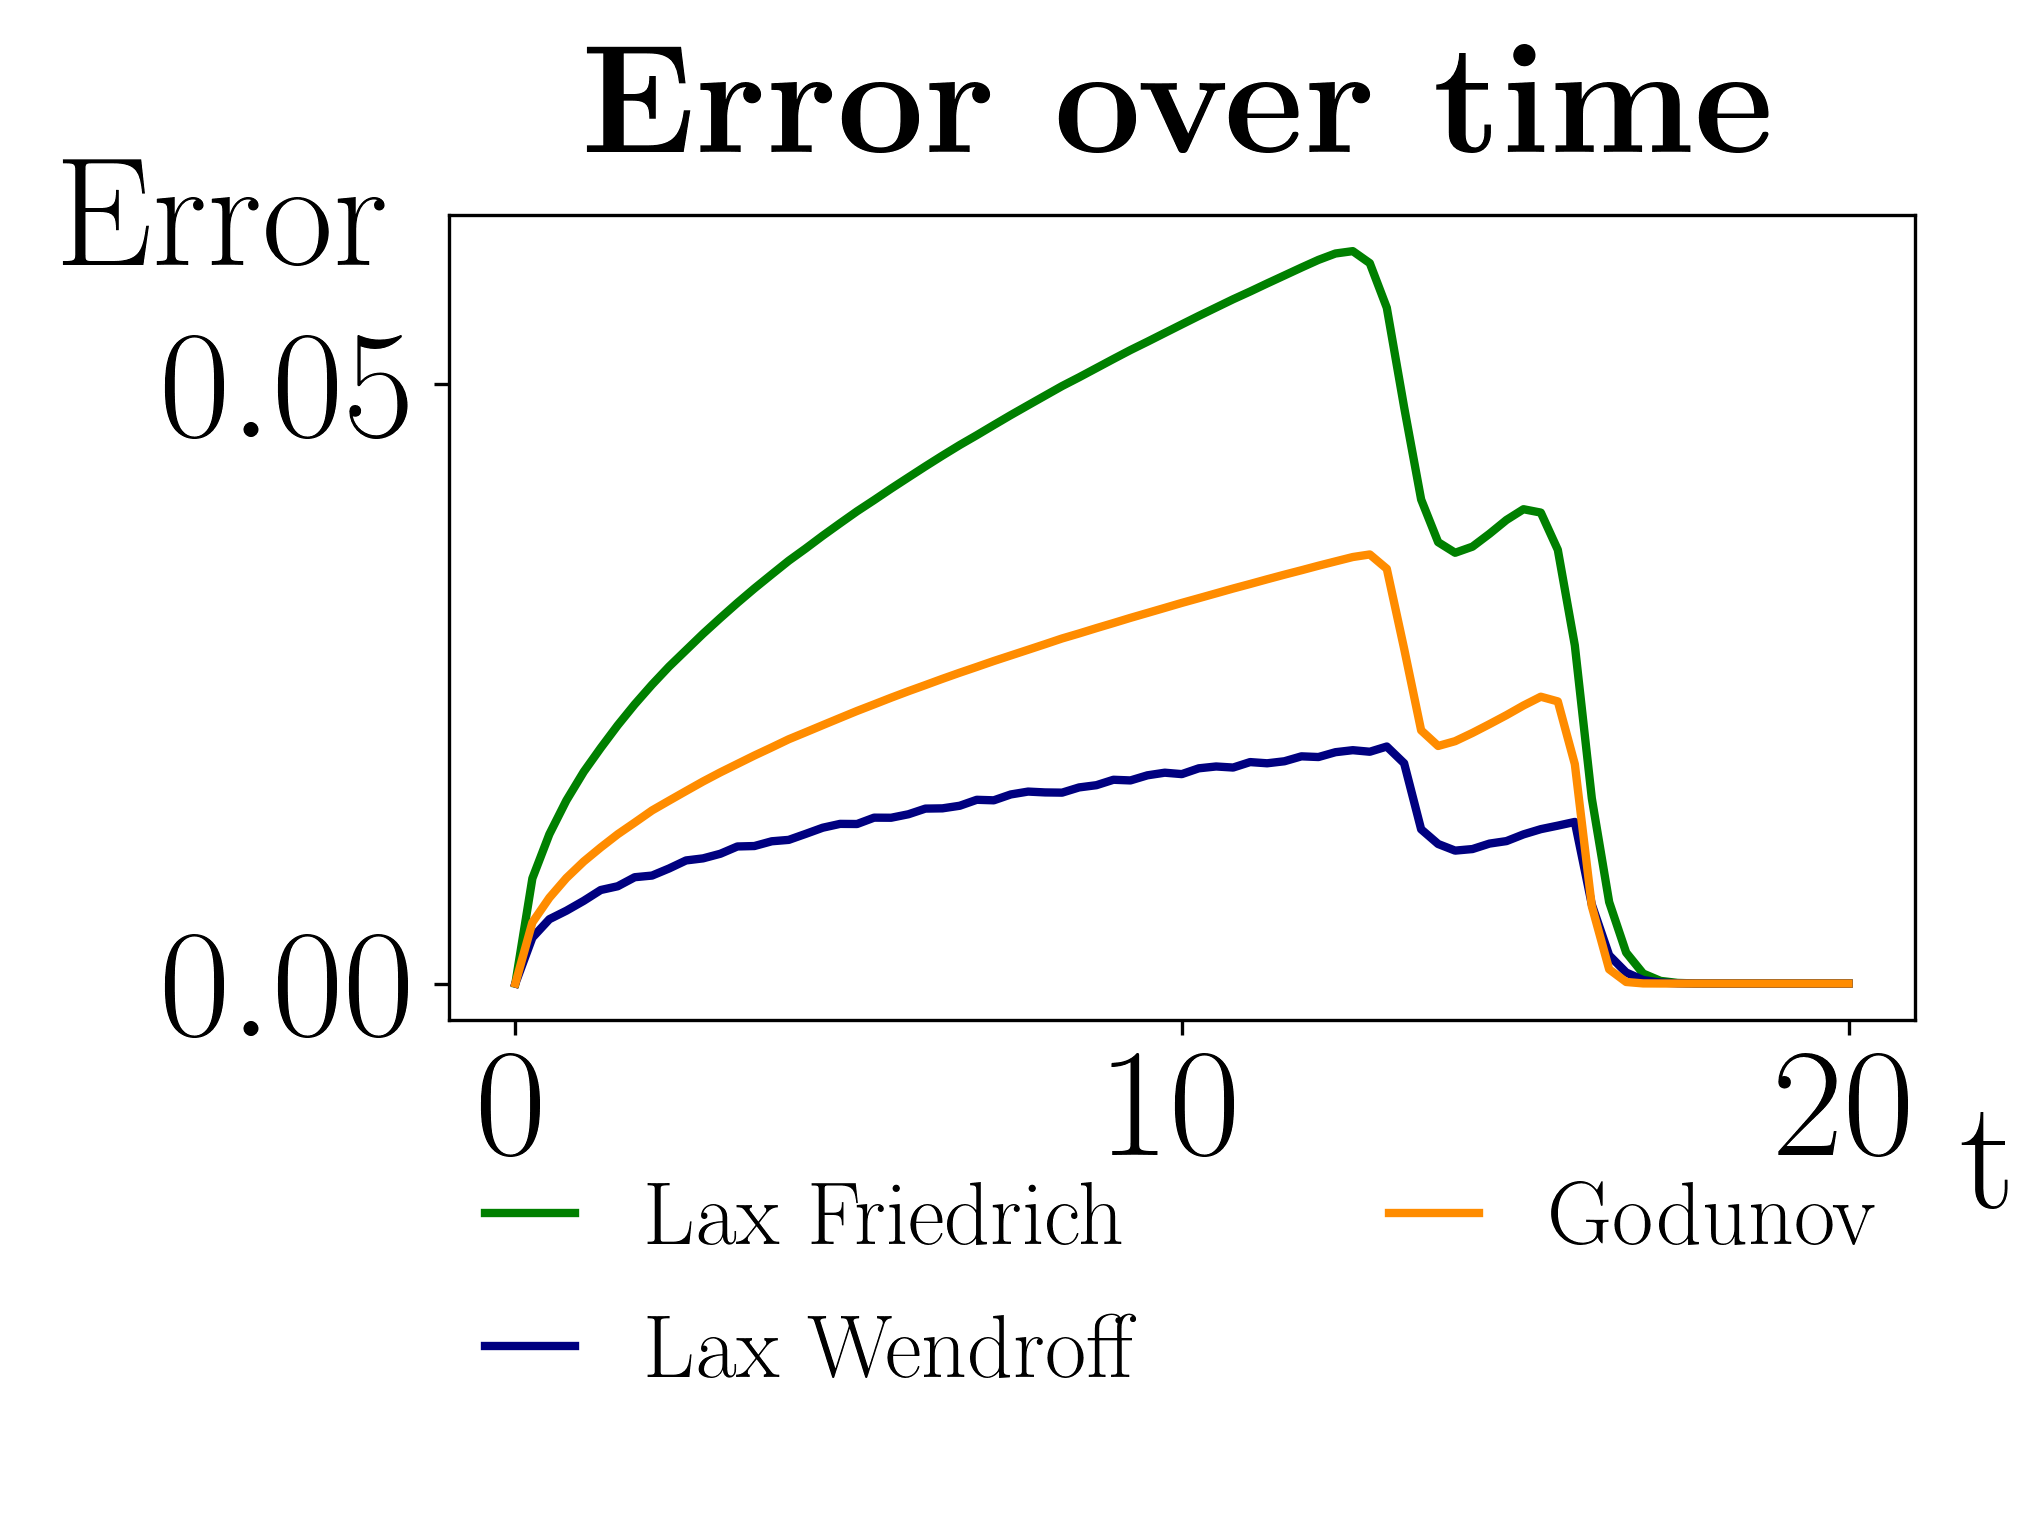
\includegraphics{fig/error_over_time.png}
    	\caption{Error of the considered scheme over time for the problem used in \cref{img:linar_comprehension}.}
    	\label{img:error_over_time}
    \end{figure}

We will now look into some non-linear advection equations. The traffic flow and the Burger's equation. The solutions are quite accurate and we can see similar behavior like the oscillations of Lax-Wendroff close to the discontinuity.

\begin{figure}
	\begin{subfigure}{\textwidth}
	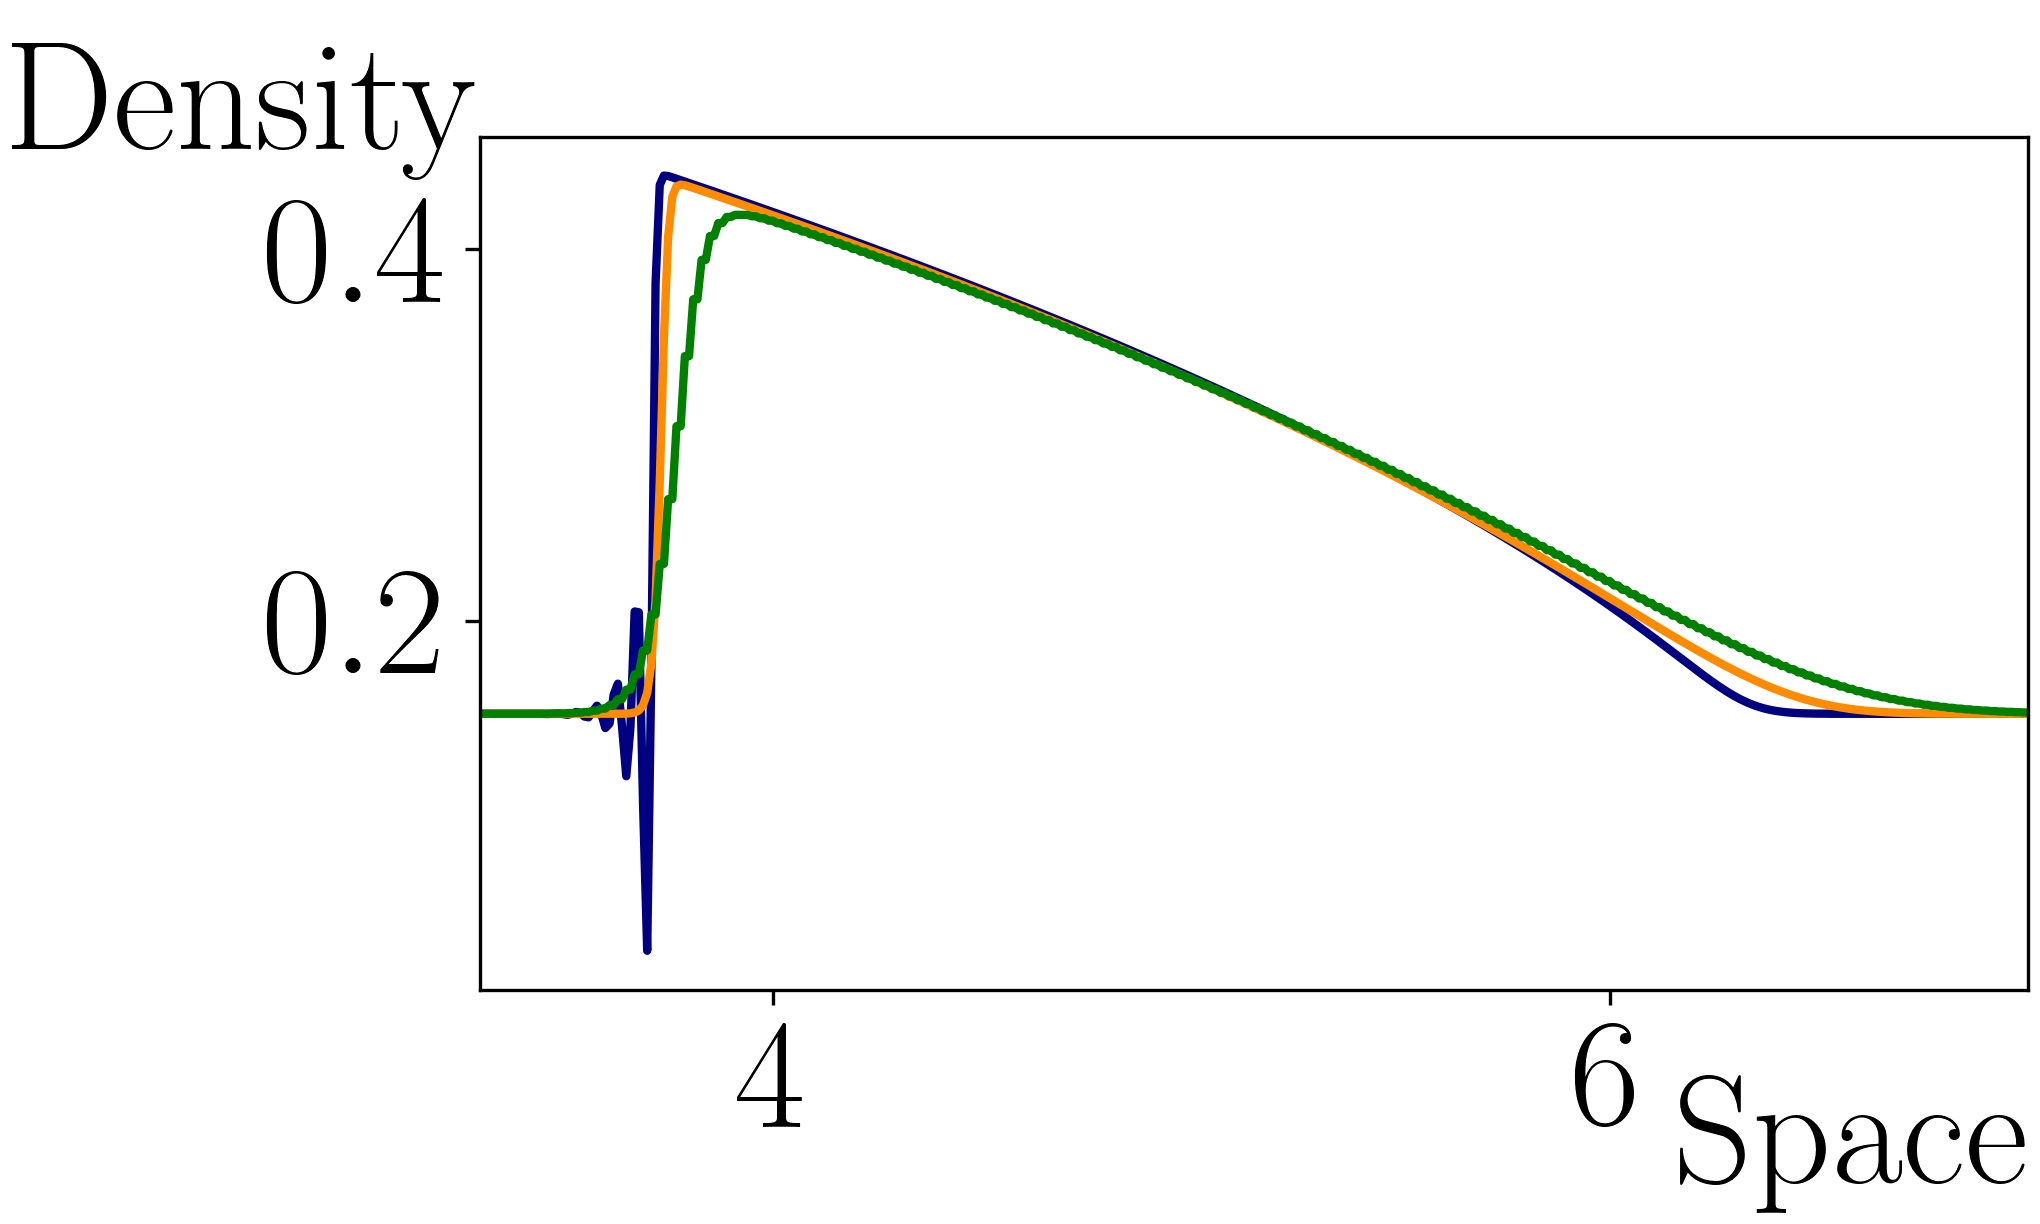
\includegraphics{fig/traffic_compare_.png}
	\caption{Traffic equation}
	\label{img:traffic_comprehension}
	\end{subfigure}

	\begin{subfigure}{\textwidth}
		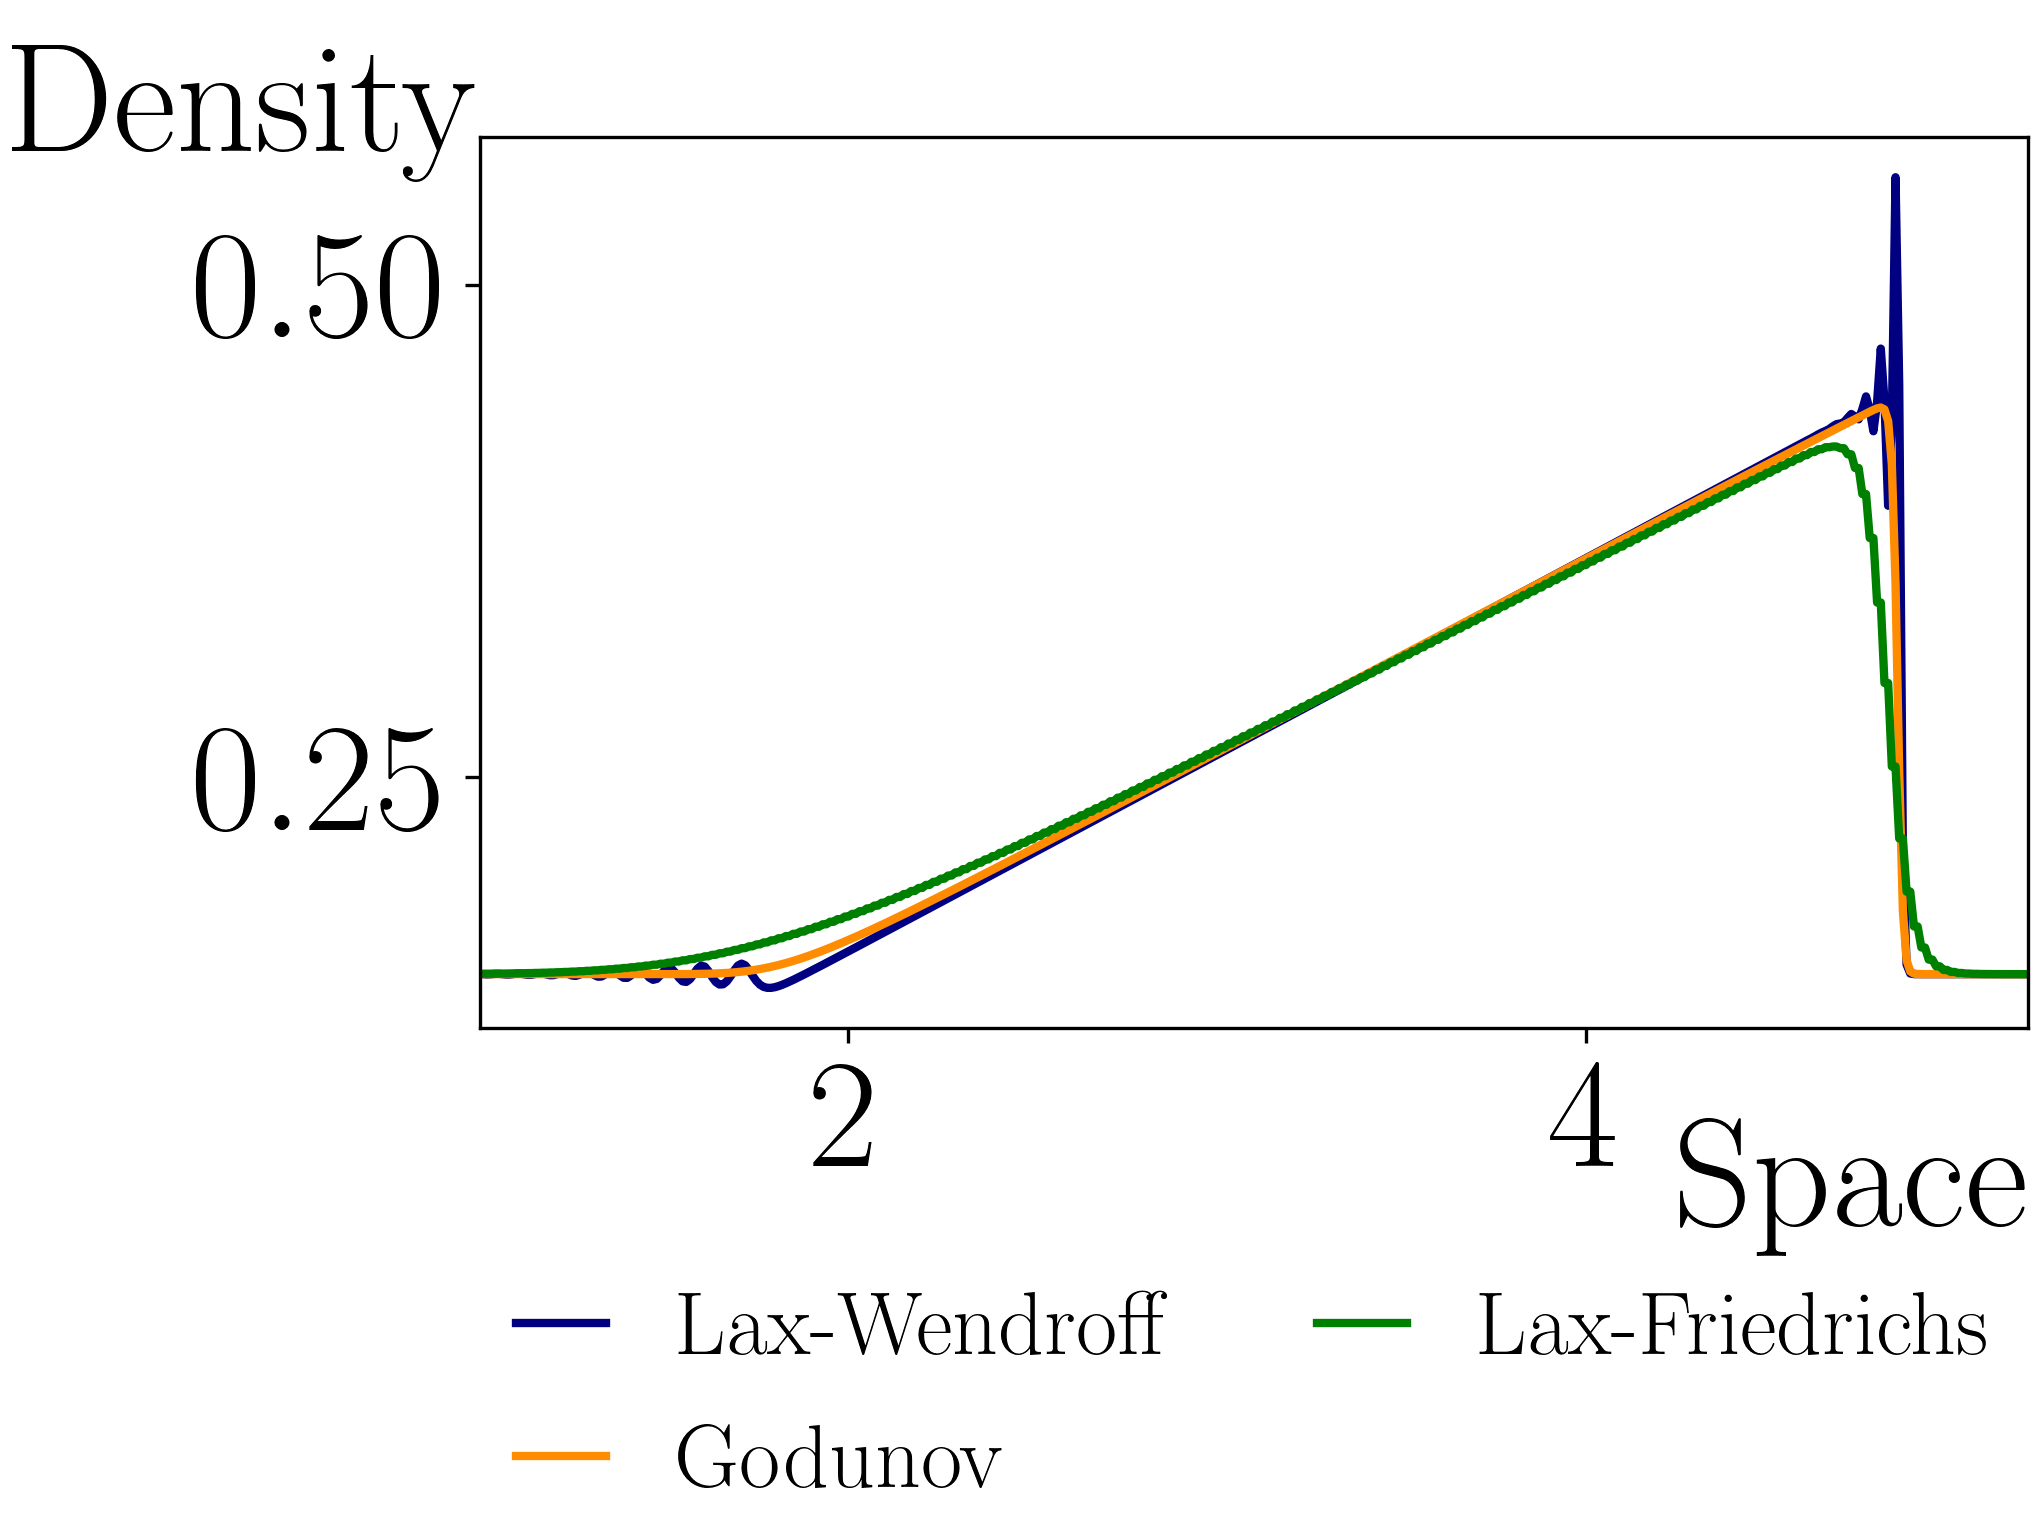
\includegraphics{fig/burger_compare.png}
		\caption{Burger's equation}
		\label{img:burger_comprehension}
	\end{subfigure}
	\caption{Approximations for the advection equaion with different flows after some time.}
\end{figure}

\textbf{Conclusion}

\vspace{0.5cm}
With the Lax-Wendroff method it is possible to get accurate approximations of a discontinuity in short runtime. So we can conclude that the it can compete with the Godonov one, which is very used nowadays.
    
    \textbf{\scriptsize{References}}
    \vspace{0.3cm}
    \nocite{*} 
    \bibliographystyle{apacite}
    \bibliography{references}
    

\end{column}
\end{column}
\end{columns}





\end{frame}
\end{document}